\section{Antecedentes}
	
	Para esta investigación se buscaron antecedentes de alcance nacional e internacional que ayuden a guiar, sustentar y validar esta investigación.
	
	\textcite{casallas2005desarrollo}, escribieron para la revista Acción Pedagógica de la Universidad de los Andes un artículo titulado \enquote{Desarrollo básico de un Laboratorio Virtual de Control de Procesos basado en Internet}, fue desarrollado conjuntamente entre la UNET y la ULA para ser usado a través de Internet y cuyo objetivo fue desarrollar un laboratorio virtual de control de procesos para la enseñanza a distancia, permitiendo ser utilizado solo por usuarios registrados y en determinados horarios. Aunque la finalidad de la investigación acá propuesta difiere del objetivo de \citeauthor{casallas2005desarrollo}, esta servirá como ayuda para determinar las funciones más utilizadas en el área de control, así como las necesidades típicas de un laboratorio de control virtual.
	
	Adicionalmente, \textcite{salazar2019diseno}, realizo en la Universidad Técnica del Norte, Ecuador, una tesis titulada \enquote{Diseño de un sistema de riego inteligente para cultivos de hortalizas basado en Fuzzy Logic en la granja la pradera de la Universidad Técnica del Norte.} para la implementación del controlador basado en la lógica difusa utilizo, entre otros equipos, un Rasberry PI para la ejecución de Python, específicamente, hizo uso de la biblioteca Scikit-Fuzzy, la cual le permitió definir las funciones de membresía, establecer las reglas difusas, realizar los procesos de fuzzificación y defuzzificación, todo esto para una arquitectura de controlador difuso tipo Mamdani, esta tesis servirá como referencia para establecer el diseño de controladores difusos utilizando la biblioteca Scikit-Fuzzy.

	Por otro lado, \textcite{congo2018aplicaciones} realizo en la Universidad Tecnológica Israel, Ecuador, una tesis titulada \enquote{Aplicaciones del software libre Python para prácticas de laboratorio aplicado a la asignatura de tratamiento digital de señales de la Universidad Tecnológica Israel} cuyo objetivo fue desarrollar por medio del software Python y sus diferentes librerías científicas, la realización de 3 Prácticas de Laboratorio para la asignatura Procesamiento Digital de Señales de la Universidad Tecnológica Israel, al igual que la intención de este trabajo, se realizó una interfaz gráfica con el objetivo de facilitar su uso, en este caso como herramienta para el procesamiento digital de señales. Este trabajo sustenta la viabilidad de realizar una interfaz gráfica con enfoque similar en el campo de la electrónica y se utilizara como guía parcial para establecer su uso en sistemas de control.
	
	Finalmente, \textcite{cadavid2009toolbox} redacto para la revista Educación en Ingeniería de Colombia, un artículo titulado \enquote{Toolbox didáctico para el diseño y análisis de sistemas de control lineal}, cuyo objetivo es describir un toolbox realizado en MATLAB para el análisis de sistemas de control lineales, este toolbox consiste de una interfaz gráfica que permite realizar pruebas a sistemas de control como respuesta escalón, respuesta en frecuencia, análisis de estabilidad, diseño de controladores, entre otras funciones. Este articulo será de utilidad para establecer la interfaz gráfica que se pretende realizar, además, sirvió como punto de partida para determinar las funciones que debería tener un laboratorio virtual de sistemas de control, como punto adicional se puede resaltar que reafirma la utilidad de esta investigación. 
	
\section{Bases teóricas}
	
	Para poder realizar el laboratorio virtual de sistemas de control clásicos y difusos será necesario abarcar conocimientos de análisis de sistemas de control, diseño de controladores PID y controladores difusos, a continuación, se presentan los conceptos necesarios para el desarrollo de esta investigación.
	
	\subsection{Procesos}
		
		Es importante partir de la base, es por ellos que empezaremos con los procesos, \textcite{sanchez2003control} define los procesos como \enquote{[...] un bloque que se identifica porque tiene una o más variables de salida de las cuales es importante conocer y mantener sus valores}(p.$\,$153). Así, un proceso se caracteriza por tener una entrada y una salida (para procesos SISO), dicha salida deberá mantenerse alrededor de un punto de referencia dado, es decir, se debe controlar su salida.
	
	\subsection{Modelado de procesos en tiempo continuo}
	
		Un proceso puede ser representado por ecuaciones diferenciales que determinen su comportamiento dinámico en el dominio del tiempo, no obstante, trabajar con ecuaciones diferenciales es tedioso a nivel matemático, por tanto, se prefiere modelar los procesos utilizando la transformada de Laplace para llevar de una representación dinámica a una algebraica, esta ecuación algebraica se operara para llevar a una función de transferencia que represente al proceso en el dominio de la frecuencia compleja \Parencite{smith1985principles}.
	
		\subsubsection{Transformada de Laplace}
		
			La transformada de Laplace de una función dependiente del tiempo f(t) viene dada por la ecuación:
			
			\begin{equation}\label{eq:Laplace}
				F(s) = \mathcal{L}\left[f(t) \right] = \int_{0}^{\infty} f(t)e^{-st}dt
			\end{equation}
			
			Si suponemos que f(t) es un proceso cuya representación dinámica viene dada por una ecuación diferencial de la forma:
			
			\begin{equation}\label{eq:Diffeq}
				a_{2}\frac{d^{2}y(t)}{dt^{2}} + a_{1}\frac{dy(t)}{dt} + a_{0}y(t) = b_{0}x(t)
			\end{equation}
			
			Aplicando \cref{eq:Laplace} a \cref{eq:Diffeq}  y despejando la relación $Y(s)/X(s)$ para el proceso con condiciones iniciales igual a cero (debido a que el proceso debe ser lineal) se obtiene la correspondiente función de transferencia del proceso $H(S)$:
			
			 \begin{equation}\label{eq:TransferFunction}
			 	H(s) =	\frac{Y(s)}{X(s)} = \frac{b_{0}}{a_{2}s^{2} + a_{1}s + a_{0}}
			 \end{equation}
			 
			 La demostración completa \Parencite[pp.$\,$21-22]{smith1985principles} no es de interés para este trabajo, pero si su resultado, la función de transferencia puede ser analizada para determinar las características del proceso, como su ganancia, constante de tiempo, tiempo muerto, entre otras.
			 
		 \subsubsection{Ecuaciones de espacio de estado}
		 
		 	Las ecuaciones de espacio de estado son un método más moderno para modelar todo tipo de sistemas, no solo físicos, sino también biológicos, económicos, sociales y otros. Así como una ecuación diferencial puede ser representada como una función de transferencia también se puede representar como una ecuación de espacio de estado, por tanto, una función de transferencia también puede ser representada en el espacio de estados y viceversa. Las ecuaciones linealizadas alrededor de un estado de operación \Parencite[p.$\,$31]{ogata2003ingenieria} son:
		 
			\begin{align}\label{eq:SSrepresentation}
				\dot{x}(t) &= A(t)x(t) + B(t)u(t) \\
				y(t) &= C(t)x(t) + D(t)u(t)
			\end{align}
			
			\begin{spacing}{1.5}
				con: 
				
				$A(t)$: como matriz de estado.
				
				$B(t)$: como matriz de entrada.
				
				$C(t)$: como matriz de salida.
				
				$D(t)$: como matriz de transmisión directa.
				
			\end{spacing}
			
			Para un modelo continuo e invariante en el tiempo las matrices A, B, C y D deben ser independientes del tiempo.
			
	\subsection{Modelado de procesos en tiempo discreto}
	
		Así como para tiempo continuo se utilizan ecuaciones diferenciales, en el tiempo discreto se hace uso de ecuaciones en diferencias, las ecuaciones en diferencias se pueden utilizar para aproximar a las ecuaciones diferenciales, estas primeras se suelen utilizar porque son más fáciles de programar \Parencite{kuo1996sistemas}.
	
		\subsubsection{Transformada z}
		
			En tiempo discreto se puede modelar un proceso utilizando la transformada z sobre la ecuación en diferencias del proceso para obtener la función de transferencia discreta $H(z)$, la ecuación general para la transformada z es:
			
			\begin{equation}\label{eq:Ztransform}
				F(z)= \sum\limits_{k=0}^{\infty}f(k)z^{-k}
			\end{equation}
			
			De este modo aplicando \cref{eq:Ztransform} sobre la entrada y salida de la ecuación en diferencias del proceso se obtiene $H(z)$ y viene dada por:
			
			\begin{equation}\label{eq:ZTransfer}
				H(z) =	\frac{Y(z)}{X(z)} = \frac{\displaystyle\sum\limits_{k=0}^{\infty}y(k)z^{-k}}{\displaystyle\sum\limits_{k=0}^{\infty}x(k)z^{-k}}
			\end{equation}
		
		\subsubsection{Ecuaciones de espacio de estado discretas}
			
			Similar al tiempo continuo, un proceso puede ser modelado utilizando ecuaciones de espacio de estado discreta, un proceso invariante en el tiempo viene dado por las siguientes ecuaciones:
			
			\begin{align}\label{eq:SSdiscreto}
				\dot{x}(k+1) &= Ax(k) + Bu(k) \\
				y(k) &= Cx(k) + Du(k)
			\end{align}
		
	\subsection{Sistemas de control}
		
		\subsubsection{Sistema en lazo abierto}
		
			Un sistema en lazo abierto es aquel cuya salida no es medida en ningún momento en orden de ajustar la entrada, esto provoca que \enquote{las perturbaciones que se presentan en el proceso ocasionen que sus efectos se sientan en la salida del proceso, es decir, en el valor de la variable controlada}\Parencite[p.$\,$350]{maloney2006electronica}. La mayoría de los sistemas en lazo abierto son estables, pero carecen de utilidad al no poder mantenerlos en un punto de referencia debido a las perturbaciones.
		
		\subsubsection{Sistema en lazo cerrado}
		
			Los sistemas de lazo cerrado son aquellos cuya salida es realimentada a la entrada del sistema, esta realimentación es de tipo negativa para que sea estable, no obstante, existen sistemas que se vuelven inestables con el simple hecho de cerrar el lazo, un ejemplo de sistema realimentado se puede observar en la \cref{fig:LazoCerrado}.
			
			\begin{figure}[htb]
				\centering
				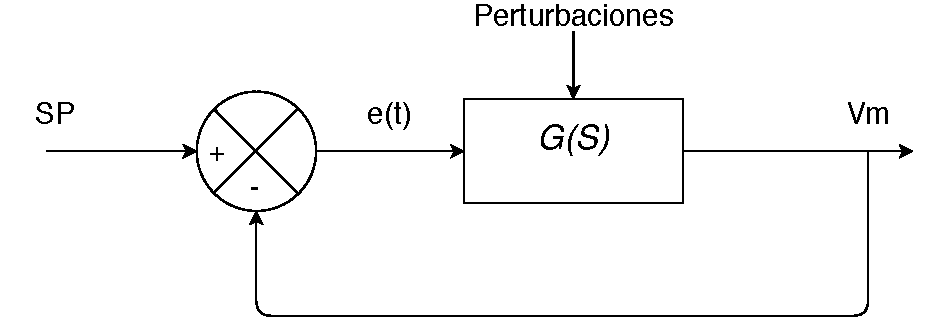
\includegraphics[width=0.66\textwidth]{LazoCerrado.pdf}
				\caption[Ejemplo de un sistema en lazo cerrado]{\textbf{Sistema en lazo cerrado}. Se observan las principales señales de un sistema en lazo cerrado. Fuente: Elaboración propia.} 
				\label{fig:LazoCerrado}
			\end{figure}
			
			En la \cref{fig:LazoCerrado} se denotan algunas de las señales que componen a un sistema de control, SP, que corresponde al set point o valor de referencia, Vm, que corresponde a la variable medida y es la variable a controlar, las perturbaciones, las cuales son magnitudes físicas que pueden afectar al proceso como la temperatura ambiente, presión, vibraciones, entre otras, y finalmente, e(t), que corresponde a la señal de error la cual viene dada por la diferencia entre el valor de referencia y la variable medida \Parencite{maloney2006electronica}.
			
%			\begin{equation}\label{eq:Serror}
%				e(t) = SP - Vm
%			\end{equation}
			
		\subsubsection{Estabilidad de los sistemas}

		La estabilidad se ve afectada por la estructura del sistema, por tanto, se debe tomar en cuanta cuando se cierra el lazo del sistema. \textcite{ogata2003ingenieria} afirma que, desde el punto de vista de estabilidad, el sistema de control en lazo abierto no es un problema importante. Por otra parte, la estabilidad es un gran problema en el sistema de control en lazo cerrado debido a la posibilidad de que se generen oscilaciones. Esto quiere decir que los análisis de estabilidad se realizan para sistemas en lazo cerrado, esto es principalmente porque los sistemas en lazo abierto tienden a ser estables, además, para realizar el control de un proceso se suele utilizar los sistemas en lazo cerrado.

			\paragraph{Análisis de estabilidad en el plano complejo}
			
				La estabilidad de un sistema lineal viene dada por la ubicación de sus polos a lo largo del plano complejo s, tomando esto en cuenta se puede determinar si un sistema en lazo cerrado es estable si no posee ninguno polo en el semiplano derecho del plano complejo s incluyendo el eje coordenado $j\omega$ \Parencite{ogata2003ingenieria}. Esto permite que el análisis de estabilidad se pueda realizar de forma analítica y gráfica.
			
			\paragraph{Criterio de estabilidad de Nyquist}
				
				El criterio de estabilidad de Nyquist determina el estado de estabilidad utilizando los polos en lazo abierto y la respuesta en frecuencia del sistema en lazo abierto, este criterio \enquote{es útil en la ingeniería de control, debido a que permite determinar gráficamente la estabilidad absoluta del sistema en lazo cerrado a partir de las curvas de respuesta en frecuencia en lazo abierto, sin que sea necesario determinar los polos en lazo cerrado}\Parencite[p.$\,$446]{ogata2003ingenieria}. Este criterio tiene la ventaja de poder realizarse tanto con cálculos analíticos como con datos experimentales.
			
			\paragraph{Análisis de estabilidad con las trazas de Bode}

				Los diagramas de bode son una forma de representar la respuesta en frecuencia de un sistema tomando en cuenta los cambios de amplitud de $H(j\omega)$ y del ángulo de fase de $H(j\omega)$ respecto a la frecuencia \Parencite{nilsson1995circuitos}. Para analizar la estabilidad se utilizan el margen de ganancia y el margen de fase del sistema en un diagrama de Bode a modo de trazas, creando así, zonas claramente delimitadas por estas trazas que determinan la estabilidad relativa del sistema dependiendo de la zona en donde se ubique en función de $\omega$.

		\subsubsection{Controlador PID}

			El controlador será el elemento dentro del sistema de control que se encargara de llevar al proceso a un valor de referencia deseado, existen varios esquemas de control para el control de procesos, cada uno con sus ventajas y desventajas, el más común es un sistema en lazo cerrado con controlador, este se puede observar en la \cref{fig:ControladorLazoCerrado}.

			\begin{figure}[htb]
				\centering
				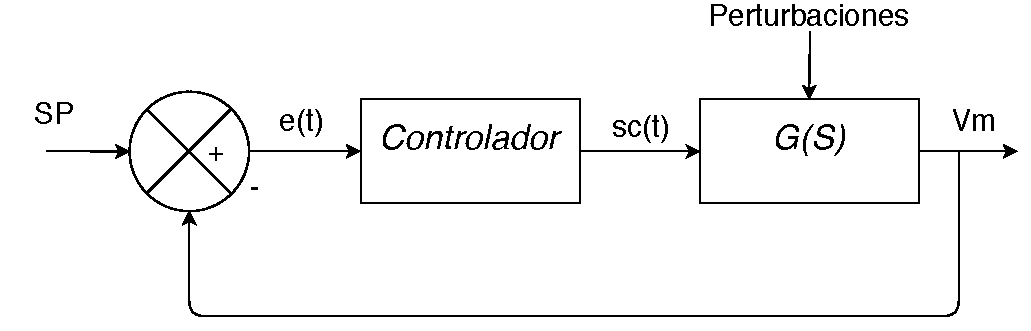
\includegraphics[width=0.66\textwidth]{LazoControlador.pdf}
				\caption[Ejemplo de un sistema en lazo cerrado con controlador]{\textbf{Sistema en lazo cerrado con controlador}. El controlador recibe la señal de error y genera una señal de control. Fuente: Elaboración propia.} 
				\label{fig:ControladorLazoCerrado}
			\end{figure}
			
			En este esquema se observa que el controlador recibe la señal de error producto del comparador entre el setpoint y la variable controlada, este error es utilizado por el controlador para generar una señal de control sc(t). El controlador más usado en la industria es el controlador PID, así lo afirma \textcite{kuo1996sistemas}: \enquote{[...] uno de los controladores más ampliamente empleados es el controlador PID [...] donde las letras son las iniciales de proporcional, integral y derivativo}(p.$\,$671). La ecuación que define a un PID en el dominio del tiempo es la siguiente:
			
			\begin{equation}\label{eq:pidtiempo}
				sc(t) = K_{p}e(t)+  K_{i}\int_{0}^{t} e(\tau) d\tau + K_{d} \frac{d}{dt}e(t)
			\end{equation}
			
			Y su forma en función de transferencia:
			
			\begin{equation}\label{eq:pidcompleja}
				G_{c}(s) = \frac{sc(s)}{e(s)} = \frac{K_{d}s^{2} + K_{p}s +  K_{i}}{s}
			\end{equation}
			
			\paragraph{Componente proporcional}

				La componente proporcional se obtiene de multiplicar la señal de error por la ganancia proporcional, esto provoca que la señal de control sea proporcional a la señal de error con una relación igual a la ganancia proporcional, si el controlador solo constase de componente proporcional el error en estado estable nunca se eliminaría, dicho de otro modo, el error podría ser muy bajo, pero jamás cero. \enquote{Este error se denomina la desviación permanente u \enquote{offset}. El mismo disminuye si se aumenta el valor de K}\Parencite[p.$\,$54]{nelson1999fundamentos}.

			\paragraph{Componente integral}

				La componente integral viene dada por la sumatoria de la señal del error en el tiempo multiplicada por la ganancia integral, por tanto, se obtiene una acumulación en un periodo determinado, esto implica que mientras exista error, la componente integral seguirá aumentando o disminuyendo dependiendo del signo de la señal de error hasta que el error sea cero, la componente integral se suma con la componente proporcional formando una única señal de control.

				Debido a que la componente integral depende del tiempo, es posible corregir desviaciones de la variable controlada generadas por perturbaciones externas, por otro lado, debido a que eventualmente se conseguirá que el error sea igual a cero la componente proporcional no hará ningún aporte al sistema, y la señal de control pasara a ser totalmente generada por la componente integral hasta que exista un cambio en el setpoint o una alteración en la variable medida.

			\paragraph{Componente derivativa}

				\looseness=-1
				La componente derivativa viene dada por el ritmo de cambio de la señal de error multiplicado por la ganancia derivativa, por tanto, cuando el error permanece constante la componente derivativa es igual a cero, la componente derivativa será tan grande como la velocidad con la que cambie el error, esto ayuda a evitar que se generen sobre pasos en la variable medida respecto a la variable de referencia.
				
				La componente derivativa es muy sensible al ruido, es por esto que se debe utilizar solo cuando se requiera un cierto grado de anticipación y no exista ruido \Parencite{smith1985principles}. Es recomendable utilizar filtros en orden de disminuir el posible ruido, a su vez, cuando el proceso a controlar es de respuesta rápida se recomienda no agregar componente derivativa o que su ganancia sea muy pequeña.
				
		\subsubsection{Entonación por método de Ziegler-Nichols en lazo abierto}
			
			El método de Ziegler-Nichols en lazo abierto requiere primero aproximar el modelo del proceso como una función de transferencia de primer orden con tiempo muerto.
			
			\begin{equation}\label{eq:firstorderProcess}
				G(s) = \frac{K}{\tau s + 1} e^{-\alpha s}
			\end{equation}
			
			Los parámetros correspondientes pueden ser obtenidos realizando una prueba al escalón y extrayendo los datos correspondientes de la gráfica de la respuesta, un ejemplo se puede observar en la \cref{fig:ZNtest}. Acá se observa: (a) $t_{0}$ que corresponde al inicio del escalón, (b) $t_{1}$ inicio de la respuesta por parte del proceso al escalón, (c) $t_{2}$ cuando el proceso alcanza el 63\% del cambio total, (d) $\Delta y$ cambio total del proceso ante el escalón y (e) $\Delta u$ magnitud de cambio de la entrada. Los parámetros para aproximar el proceso a un modelo de primer orden con tiempo muerto se calculan como sigue:
			
			\begin{align}\label{eq:parametros}
				K &= \frac{\Delta y}{\Delta u}\\
				\tau &= t_{2} - t_{1}\\
				\alpha &= t_{1} - t_{0}
			\end{align}
			
			\begin{figure}[p]
				\centering
				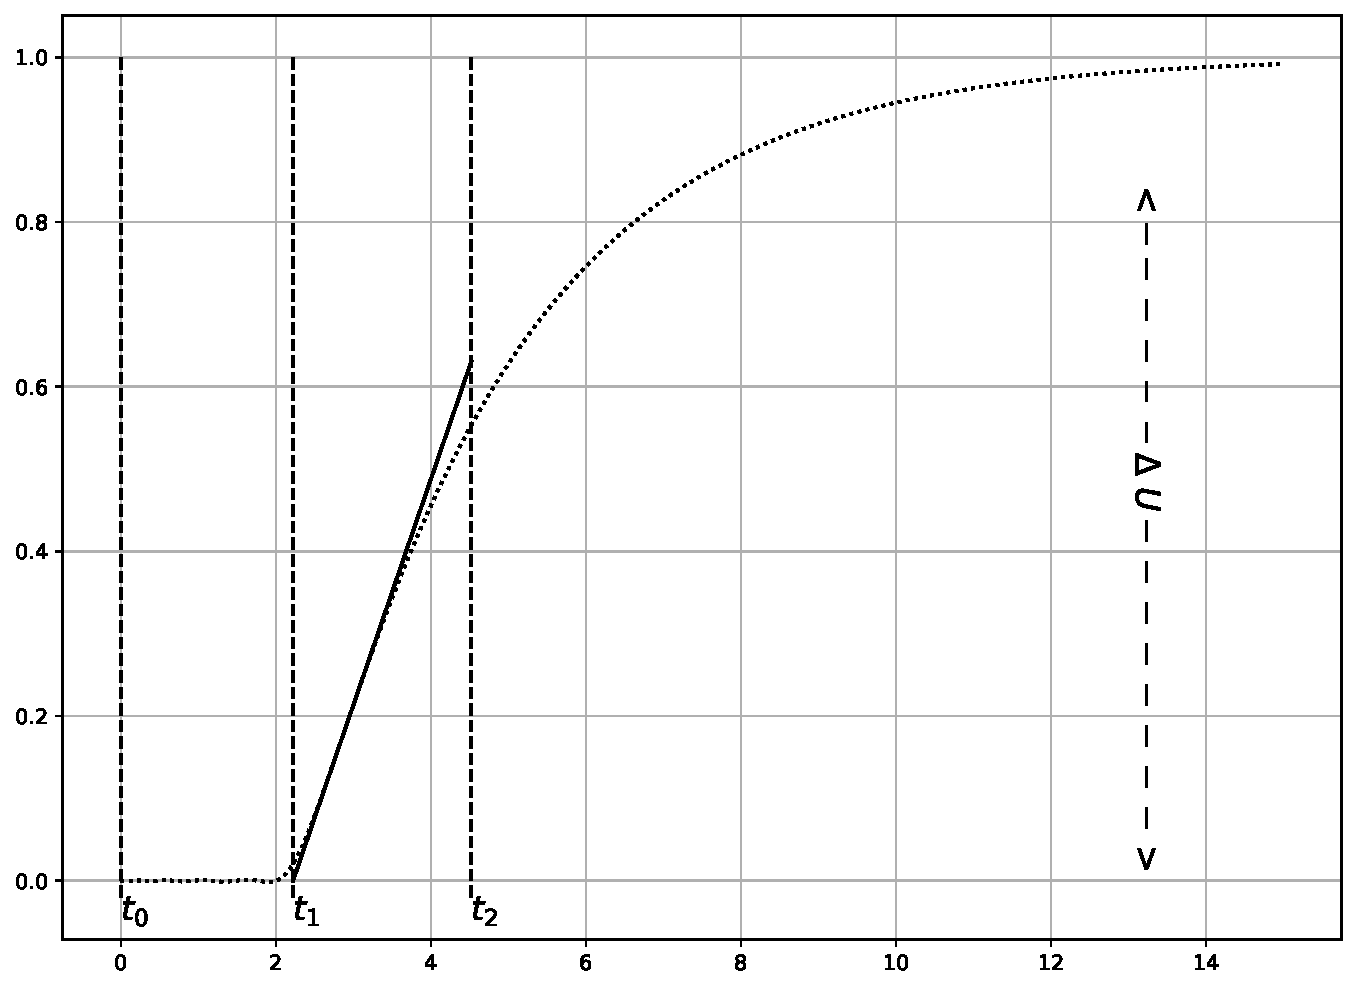
\includegraphics[width=0.9\textwidth]{ZieglerN.pdf}
				\caption[Modelado por curva de reacción]{\textbf{Modelado por curva de reacción.} Para realizar este modelado se estudia la respuesta del sistema ante la entrada de la función de heaviside u(t), también llamada función escalón unitario, el modelo obtenido a través de este método es una aproximación del sistema. Fuente: Elaboración propia.} 
				\label{fig:ZNtest}
			\end{figure}
			
			Con estos valores se puede obtener la entonación de un controlador P, PI o PID, los valores de $K_{p}$, $K_{i}$ y $K_{d}$ se pueden obtener sustituyendo los valores en la \cref{tab:ZiglerNichols} correspondiente a la regla de entonación de Ziegler-Nichols. \textcite{ogata2003ingenieria} comenta que: \enquote{Las reglas de sintonía de Ziegler-Nichols [...] se han usado ampliamente para sintonizar controladores PID en sistemas de control de procesos en los que no se conoce con precisión la dinámica de la planta}(p.$\,$572).
			
			% Plantilla para tabla ajustada al texto
			\begin{table}[p]
				\centering
				\begin{threeparttable}
					\renewcommand{\arraystretch}{2.5} 	% Separacion de las filas
					%\setlength{\tabcolsep}{6pt}			% Separacion de columnas
					\caption[Regla de entonación de Zigler-Nichols]{Regla de entonación de Zigler-Nichols}
					\begin{tabular*}{\textwidth}{c @{\extracolsep{\fill}}ccc}
						\toprule
						Tipo de controlador & $K_{p}$                               &              $T_{i}$              &         $T_{d}$          \\ \midrule
						         P          & $\displaystyle\frac{\tau}{\alpha}$    &       $\displaystyle\infty$       &            0             \\
						        PI          & $0.9\displaystyle\frac{\tau}{\alpha}$ & $\displaystyle\frac{\alpha}{0.3}$ &            0             \\
						        PID         & $1.2\displaystyle\frac{\tau}{\alpha}$ &      $2\displaystyle\alpha$       & $0.5\displaystyle\alpha$ \\ \bottomrule
					\end{tabular*}
					\label{tab:ZiglerNichols}
					\begin{tablenotes}[flushleft]
						\item {\footnotesize \textbf{Nota.} Los valores de $K_{i}$ y $K_{d}$ se pueden obtener de la siguiente forma: $K_{i} = K_{p}/T_{i}$ ; $K_{d} = K_{p}T_{d}$. Fuente: \textcite{ogata2003ingenieria}.}
					\end{tablenotes}
				\end{threeparttable}
			\end{table}
			
	\subsection{Lógica difusa}
		
		La lógica difusa es una extensión matemática de la lógica convencional en donde se asigna un grado de pertenencia a un hecho entre un valor verdadero y uno falso, \enquote{consiste en que los valores verdaderos (en lógica difusa) o valores de pertenencia (en conjuntos difusos) se indican en un número entre [0.0, 1.0], donde 0.0 representa falsedad total y 1.0 significa verdad absoluta}\Parencite[p.$\,$4]{cruz2010inteligencia}.
		
		La lógica se puede estructurar en tres etapas, la primera etapa consiste en establecer cada una de las variables con etiquetas lingüística que determinen en conjunto el universo de discurso de cada una de ellas, es decir, se crean los conjuntos difusos, en la segunda etapa se definen las reglas de inferencia difusa que determinaran el comportamiento del sistema difuso, y tercera, se obtienen los valores de salida utilizando las reglas de inferencia y realizando el proceso de defuzzificación que consiste en llevar los grados de pertenencia a un valor nítido o real \Parencite{cruz2010inteligencia}.
		
		\subsubsection{Conjuntos difusos}
			
			Un conjunto difuso está compuesto de funciones de membresía, dichas funciones de membresía representan valores para asignar el grado de pertenencia de una variable a un estado en particular, estos estados son identificados con etiquetas lingüísticas descriptivas, como alto, caliente, bajo, negativo, entre otras, en la \cref{fig:FuzzySet} se puede observar un ejemplo de conjunto difuso.
			
			\begin{figure}[htb]
				\centering
				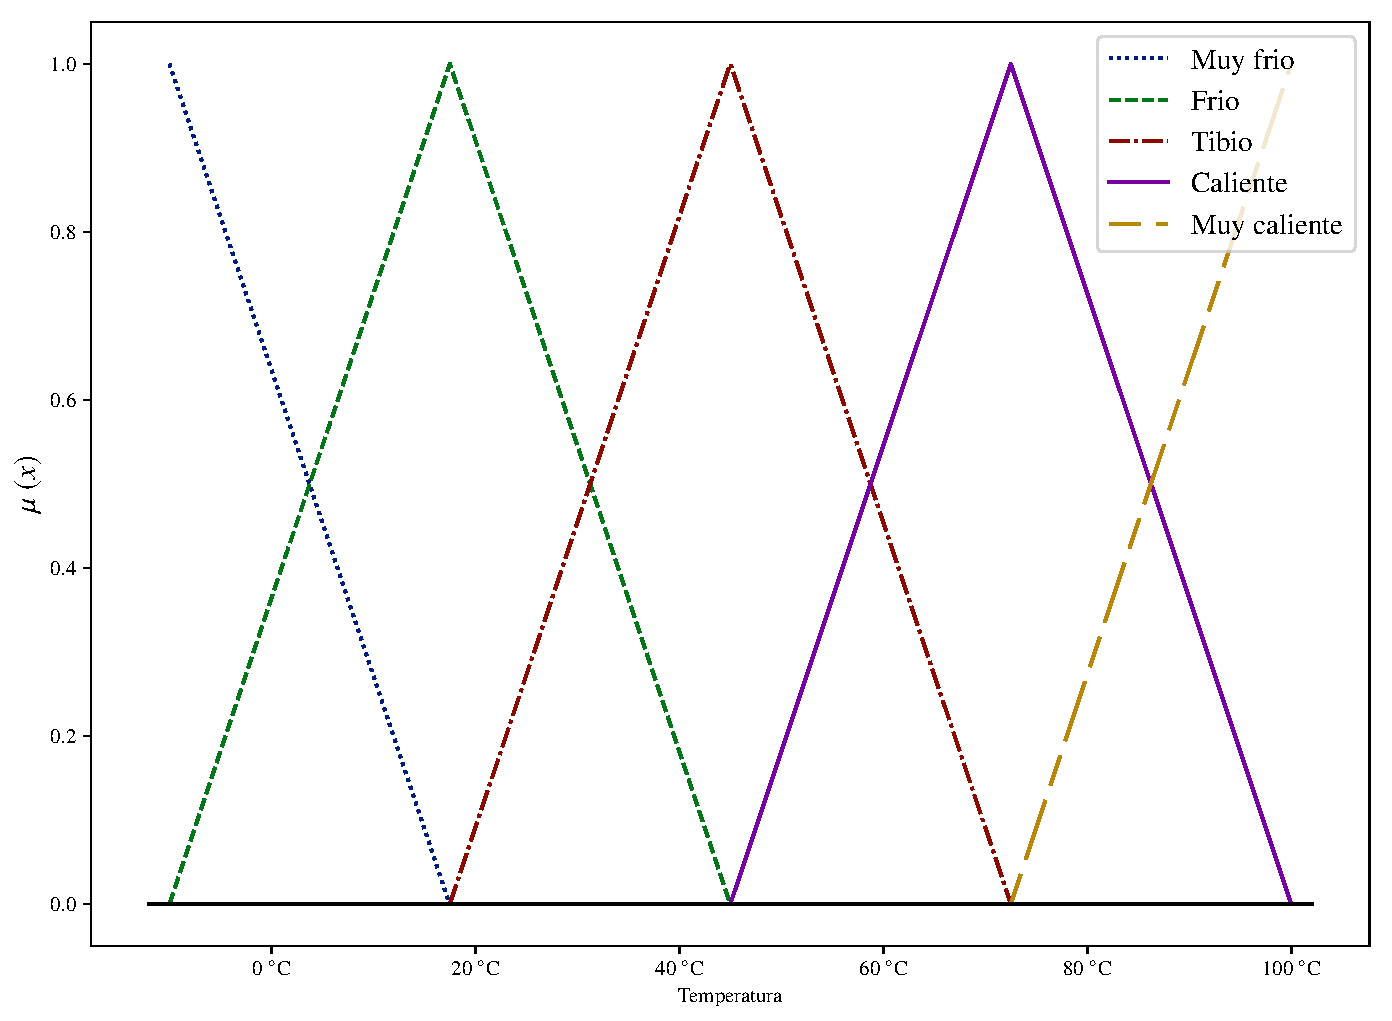
\includegraphics[width=0.55\textwidth]{FuzzySet.pdf}
				\caption[Ejemplo de un conjunto difuso]{\textbf{Ejemplo de un conjunto difuso}. Este conjunto difuso corresponde a una variable de temperatura que va desde -10\textdegree C hasta 100\textdegree C. Fuente: Elaboración propia.} 
				\label{fig:FuzzySet}
			\end{figure}
			
			Las funciones de membresía pueden tomar varias formas y rangos en orden de poder representar de mejor forma los grados de pertenencia de la variable a una etiqueta en particular, sin embargo, las formas triangulares suelen ser las menos pesadas en memoria y en poder de computo \Parencite{riid2003transparent}. La cantidad de etiquetas que se pueden asignar a un conjunto difuso es ilimitada, pero se debe tener en cuenta el nivel de complejidad que se genera a medida que se incrementa su número.
			
		\subsubsection{Reglas de inferencia}
			
			Las reglas de inferencia, al igual que en la lógica convencional, se encargan de realizar una conexión entre los antecedentes y los consecuentes con el fin de obtener una salida, en este caso, entre los conjuntos difusos de entrada y la salida, la salida puede ser un conjunto difuso o una función matemática. Como sugiere \textcite{cruz2010inteligencia}, las reglas pueden formularse de dos formas denominadas modus ponens y modus tollens, modus ponens utiliza los antecedentes para obtener el consecuente, por otro lado, el modus tollens utiliza los consecuentes recíprocos para obtener el antecedente. La tautología para modus ponens y modus tollens se puede observar a modo de tablas de la verdad en la \cref{tab:mponens} y \cref{tab:mtollens} respectivamente.
			
			\begin{table}[t]
				\centering
				\begin{threeparttable}
					\renewcommand{\arraystretch}{1.8} 	% Separacion de las filas
					%\setlength{\tabcolsep}{6pt}			% Separacion de columnas
					\caption[Tautología para modus ponens]{Tautología para modus ponens}
					\begin{tabular*}{\textwidth}{c @{\extracolsep{\fill}} cccc}
						\toprule
						A & B  & A$\rightarrow$B & (A$\wedge$(A$\rightarrow$B)) & (A$\wedge$(A$\rightarrow$B))$\rightarrow$B \\ \midrule
						0 & 0 &       1        &              0              &                     1                     \\
						0 & 1 &       1        &              0              &                     1                     \\
						1 & 0 &       0        &              0              &                     1                     \\
						1 & 1 &       1        &              1              &                     1                    \\ \bottomrule
					\end{tabular*}
					\label{tab:mponens}
				\end{threeparttable}
			\end{table}
			
			\begin{table}[t]
				\centering
				\begin{threeparttable}
					\renewcommand{\arraystretch}{1.8} 	% Separacion de las filas
					%\setlength{\tabcolsep}{6pt}			% Separacion de columnas
					\caption[Tautología para modus tollens]{Tautología para modus tollens}
					\begin{tabular*}{\textwidth}{c @{\extracolsep{\fill}} cccc}
						\toprule
						A & B  & A$\rightarrow$B & (A$\wedge$(A$\rightarrow$B)) & (A$\wedge$(A$\rightarrow$B))$\rightarrow$B \\ \midrule
						0 & 0 &       1        &              0              &                     1                     \\
						0 & 1 &       0        &              0              &                     1                     \\
						1 & 0 &       1        &              0              &                     1                     \\
						1 & 1 &       1        &              1              &                     1                    \\ \bottomrule
					\end{tabular*}
					\label{tab:mtollens}
					\begin{tablenotes}[flushleft]
						\item {\footnotesize \textbf{Nota.} La tautología para modus ponens y modus tollens es presentada utilizando tablas de la verdad. Fuente: \textcite{cruz2010inteligencia}, p.$\,$70}
					\end{tablenotes}
				\end{threeparttable}
			\end{table}
			
		\subsubsection{Defuzzificación}

			En esta última etapa también llamada desdifusificación, se obtienen los valores reales de salida, \textcite{cruz2010inteligencia} lo describe como el \enquote{[...] mapeo a escala que convierte el rango de valores de las variables de salida a sus universos de discurso correspondientes. La desdifusificación es la herramienta para obtener la acción de control nítida a partir de una acción de control difusa} (p.$\,$73). Este proceso es matemáticamente costoso y existen distintos métodos para realizarlo, el más común es el método de centro de área.
			
			\paragraph{Método de centro de área}

				Este método se utiliza para realizar la defuzzificación y obtener las salidas nítidas, consiste en cortar las funciones de membresía $\mu_{n}(x)$ con los valores de entrada $x$ para determinar un área, el área inferior será la que se tome en cuenta para realizar el cálculo, el método de centro de área se puede representar de modo general en su forma discreta de la siguiente forma:
				
				\begin{equation}\label{eq:Centroide}
					Salida = \frac{\displaystyle\sum\limits_{x=a}^{b}\mu_{n}(x)\cdot x}{\displaystyle\sum\limits_{x=a}^{b}\mu_{n}(x)}
				\end{equation}
	
		\subsubsection{Sistemas de control difusos}
			
			Un controlador difuso es cualquier tipo de controlador que utilice en su interior alguna forma de lógica difusa, al igual que con los controladores clásicos el esquema de control más común es en lazo cerrado tal como se observa en la \cref{fig:fuzzycontrollerclassic}. El controlador difuso a su vez puede contener todo tipo de metodologías de control, de hecho, el uso más común es realizar un controlador P, PI, PD o PID, todos difusos. Para realizar estos controladores se suele utilizar la estructura Mamdani, la cual asigna conjuntos difusos para las entradas y para las salidas, por tanto, es necesario el proceso de defuzzificación, comúnmente con el método de centro de área.
					
			\begin{figure}[htb]
				\centering
				\begin{subfigure}[t]{0.8\textwidth}
					\centering
					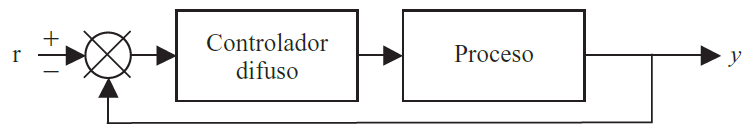
\includegraphics[width=\textwidth]{FuzzyControllerClassic} % el archivo debe estar en la carpeta imágenes
					\caption{} 
					\label{fig:fuzzycontrollerclassic}
				\end{subfigure}
				\hfill
				\begin{subfigure}[t]{0.8\textwidth}
					\centering
					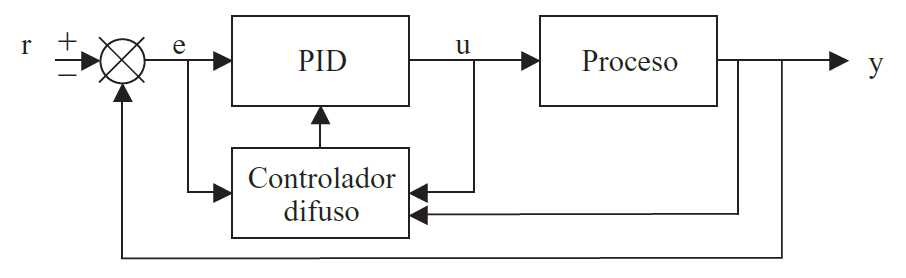
\includegraphics[width=\textwidth]{FuzzyControllerAdapt} % el archivo debe estar en la carpeta imágenes
					\caption{}
					\label{fig:fuzzycontrolleradapt}
				\end{subfigure}
				
				\caption[Esquemas de control difuso]{\textbf{Esquemas de control difuso}. (a) Esquema de control difuso clásico, (b) Esquema de control difuso autosintonizable. Fuente: \textcite{cruz2010inteligencia}, p.$\,$86 y p.$\,$104 respectivamente. \label{fig:FuzzySchems}}
			\end{figure}
			
			Adicionalmente existe el esquema de control difuso con PID autosintonizable, el cual consiste en dos controladores, uno difuso y un PID clásico, el controlador difuso se encargara de generar las ganancias del PID de forma dinámica en función de las entradas que reciba, a su vez, el PID será quien gobierne al proceso, esto permite adaptar el controlador PID a los cambios de carga y a los cambios del setpoint, el esquema de control se puede observar en la \cref{fig:fuzzycontrolleradapt}.

			No existen métodos analíticos claros para la entonación de controladores difusos, por tanto, la entonación se debe realizar bajo la experiencia del diseñador, tomando en cuenta las necesidades de control y las dinámicas del proceso, esto es debido a que el controlador difuso depende enteramente de la estructura de los conjuntos difusos y de la asignación de las reglas de inferencia \Parencite{cruz2010inteligencia}.
		
	\subsection{Python}
		
		Python es un lenguaje de programación interpretado y multiparadigma ya que soporta programación orientada a objetos, imperativa y en menor medida funcional. \textcite{guido2017tutorial} afirma que Python es un lenguaje de programación potente que puede aprenderse fácilmente. Cuenta con estructuras de datos eficientes y de alto
		nivel y un enfoque simple pero efectivo a la programación orientada a objetos. La elegante sintaxis de Python y su escritura
		dinámica, junto con su naturaleza interpretada, hacen de éste un lenguaje ideal para scripting y desarrollo rápido de
		aplicaciones en diversas áreas y sobre la mayoría de las plataformas.
		
		Adicionalmente, Python posee bibliotecas externas para realizar cálculos numéricos complejos, también existen bibliotecas para el análisis de sistemas de control y para el diseño de controladores difusos, por otro lado, existen bibliotecas para salidas gráficas con calidad de publicación, gráficas en tiempo real y en 3D.
		
		\subsubsection{Biblioteca NumPy}

			NumPy es una biblioteca para realizar cálculos computacionales científicos y matemáticos, algunas de sus funciones son: cálculo de vectores n-dimensionales, transformada de Fourier, álgebra lineal, entre otras \Parencite{numpy}

		\subsubsection{Biblioteca SciPy}	

			El paquete SciPy es un conjunto de bibliotecas matemáticas, científicas y de ingeniería compuestas por: NumPy, SciPy (biblioteca), SymPy, Matplotlib, IPython y Pandas, la biblioteca SciPy es uno de los núcleos del paquete SciPy. Provee varias rutinas eficientes de uso amigable para el usuario de tipo numérica para realizar integración, interpolación, optimización, álgebra lineal, estadísticas, entre otras \Parencite{scipy}, toda la documentación puede ser conseguida en la página oficial de SciPy.
			
		\subsubsection{Biblioteca Matplotlib}

			Matplotlib es una biblioteca para la graficación 2D que produce figuras con calidad de publicación en varios formatos y a través de múltiples ambientes interactivos. Matplotlib puede ser usado en scripting, consolas de comando, IPython, jupyter notebooks y en aplicaciones web \Parencite{Hunter:2007}. La sintaxis para usar Matplotlib es muy similar al sistema de plots de MATLAB, del mismo modo, configurar parámetros de estilos, fuentes, anchos de línea, entre otros, se realiza de manera similar.

		\subsubsection{Biblioteca de control}

			La biblioteca control de python es un conjunto de clases y funciones que implementan las operaciones más comunes en sistemas de control, además, posee un módulo de compatibilidad para usuarios de MATLAB que emula las funciones y sintaxis de este lenguaje \Parencite{pythoncontrol}. Para crear el modelo de un sistema podemos usar ecuaciones de espacio de estado o funciones de transferencia.

		\subsubsection{Biblioteca Scikit-Fuzzy}
			
			Scikit-Fuzzy es una colección de algoritmos de lógica difusa con la intención de pertenecer al paquete de herramientas científicas SciPy, esta biblioteca permite diseñar y simular controladores difusos con estructura tipo Mamdani \Parencite{warner2016fuzzy}, no posee un modo para realizar lazos de control o compatibilidad con la biblioteca de control de forma directa, de modo que se tendrían que codificar aparte las rutinas que conformen el lazo cerrado de control.
			